\chapter{Results}
As only the basic line expansion router and the extended version produce really useful results I will explain only results for these two. For the first version \nref{fig:miller_amplifier_routed_basic_line_expansion} it is quite easy to determine if the result is reasonable, as it choses always the shortest connection (or better said: the one with the smallest resistance). The two presented layouts have a relatively big minimal distance between all modules set, which causes the actually too big layout. This was necessary, as it is not yet supported by the GUI of the ICFBInterface to specify minimum distances between only some modules. Therefore, I had to choose a big minimum distance between all modules, although I needed only a bigger distance inside the common centroid.

\begin{figure}
	\centering
	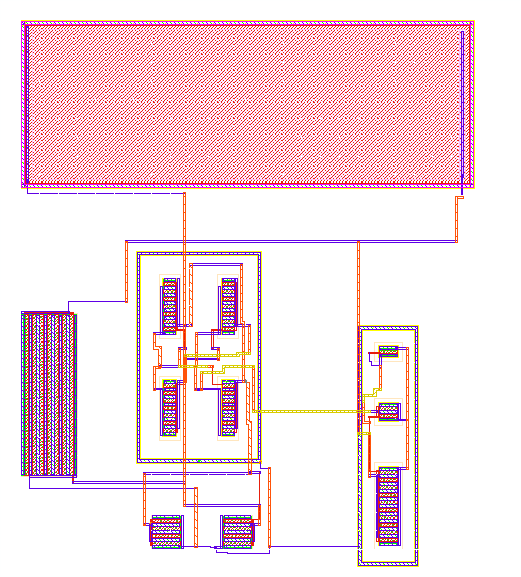
\includegraphics[scale=.6]{FIG/miller_amplifier_routed_basic_line_expansion.png}
  	\caption{routed layout of the miller amplifier, with the basic line expansion router}
	\label{fig:miller_amplifier_routed_basic_line_expansion}
\end{figure}

For the second one, the extend line expansion router, it becomes a lot more difficult to determine manually if there are errors in the layout \nref{fig:miller_amplifier_routed_extended_line_expansion}. This router decides which connection should be used also based on the capacitive couplings, therefore it mustn't be always the shortest one.

\begin{figure}
	\centering
	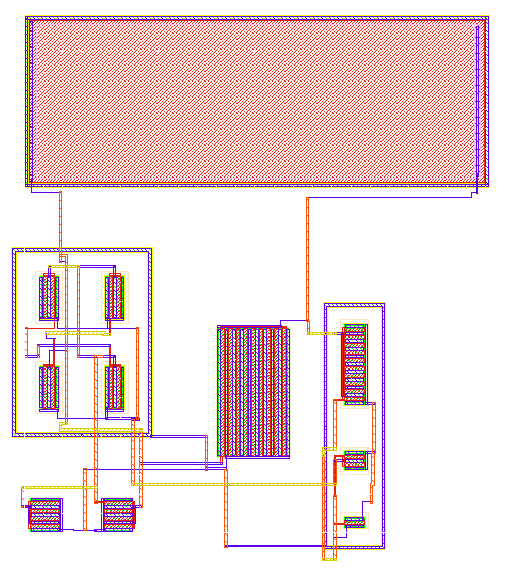
\includegraphics[scale=.6]{FIG/miller_amplifier_routed_extended_line_expansion.png}
  	\caption{routed layout of the miller amplifier, with the extended line expansion router}
	\label{fig:miller_amplifier_routed_extended_line_expansion}
\end{figure}

To show also the results of a layout with a symmetried I have prepared one simple example which contains only three modules \nref{fig:symmetry_routed}. Two of them form a pair of a symmetry and the other one is a single module in this symmetry. In the layout can be seen that the two connections between the symmetric modules are connected nearly symmetric the third module. The maximum allowed difference in resistance is 5\%, which seems to be hold by both connections. One of them is optical quite unsymmetric connected, but it starts on both ends on POLY. Therefore, the resistance of the whole connection is dominated by those two small parts.

\begin{figure}
	\centering
	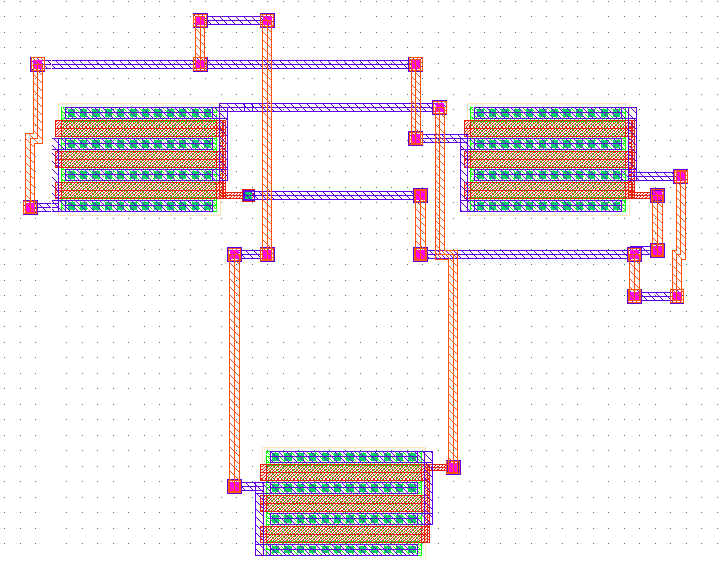
\includegraphics[scale=.6]{FIG/symmetry_routed.png}
  	\caption{routed layout of a symmetry}
	\label{fig:symmetry_routed}
\end{figure}

\section{Simulation Results}
To determine how well the extended line expansion router reduces the parasitics I have done some simulation on two layouts, which differ only in the routes. I compare all the results of the resulting amplifier with those simulation results, where no parasitics were backpropagated.

MISSING